\documentclass[12pt]{article}
\usepackage{listings}
\usepackage{url}
\usepackage{listing}
\usepackage{amsmath}
\usepackage{graphics}
\usepackage{fancyhdr}
\usepackage[dvips]{graphicx}
\usepackage[english]{babel}

\newcommand{\figw}{1\linewidth}


\DeclareMathOperator*{\mean}{mean}

\begin{document}

\begin{Large} \noindent {\bf{The DESERT Underwater Libraries:\\ Schematic Description of the Modules}} \end{Large}

\vspace{0.8cm}
\begin{abstract}
 In this document we provide a brief and schematic description of all the modules included in the first release of DESERT Underwater (version 1.0.0). The described modules are grouped according to the TCP/IP stack, from Section~\ref{sec:application} to~\ref{sec:physical}. The modules implemented to simulate node mobility are also considered, see Section~\ref{sec:mobility}.\\

 {\it Legend of the adopted scheme to describe the DESERT Underwater's modules}
 \begin{description}
    \item {\bf Name:} The name of the module;
   \item {\bf Description:} A brief description of the module capabilities and functionalities;
   \item {\bf Library name:} the name of the corresponding NS-Miracle (DESERT) library;
   \item {\bf Tcl name:} The name of the module in Tcl, i.e., the tcl command to call in order to create the corresponding C++ object;
   \item {\bf Tcl parameters:} Parameters that can be set via Tcl, their ranges and usage, i.e., what they are needed for;
   \item {\bf Tcl commands:} Commands that can be set via Tcl with a specification of the mandatory commands that must be called to make everything running properly (e.g., initialization commands);
   \item {\bf Internal packet headers:} Packet headers defined by the module (if applicable);
   \item {\bf External packet headers:} External packet headers used by the module (if applicable);
   \item {\bf Warnings:} Possible warnings for the good usage of the module, e.g., the use of this module in conjunction with module A,B,C is deprecated and/or can lead to an undefined behaviour.
   \item {\bf Parent Libraries:} Mandatory NS-Miracle/DESERT libraries that must be loaded in the Tcl file of the parameter setting before loading the library of this module.
   \item {\bf Tcl Scripts:} Name of the tcl sample where to find an usage example of the considered module;
\end{description}
\end{abstract}

\newpage

\begin{figure}[h]
\begin{center}
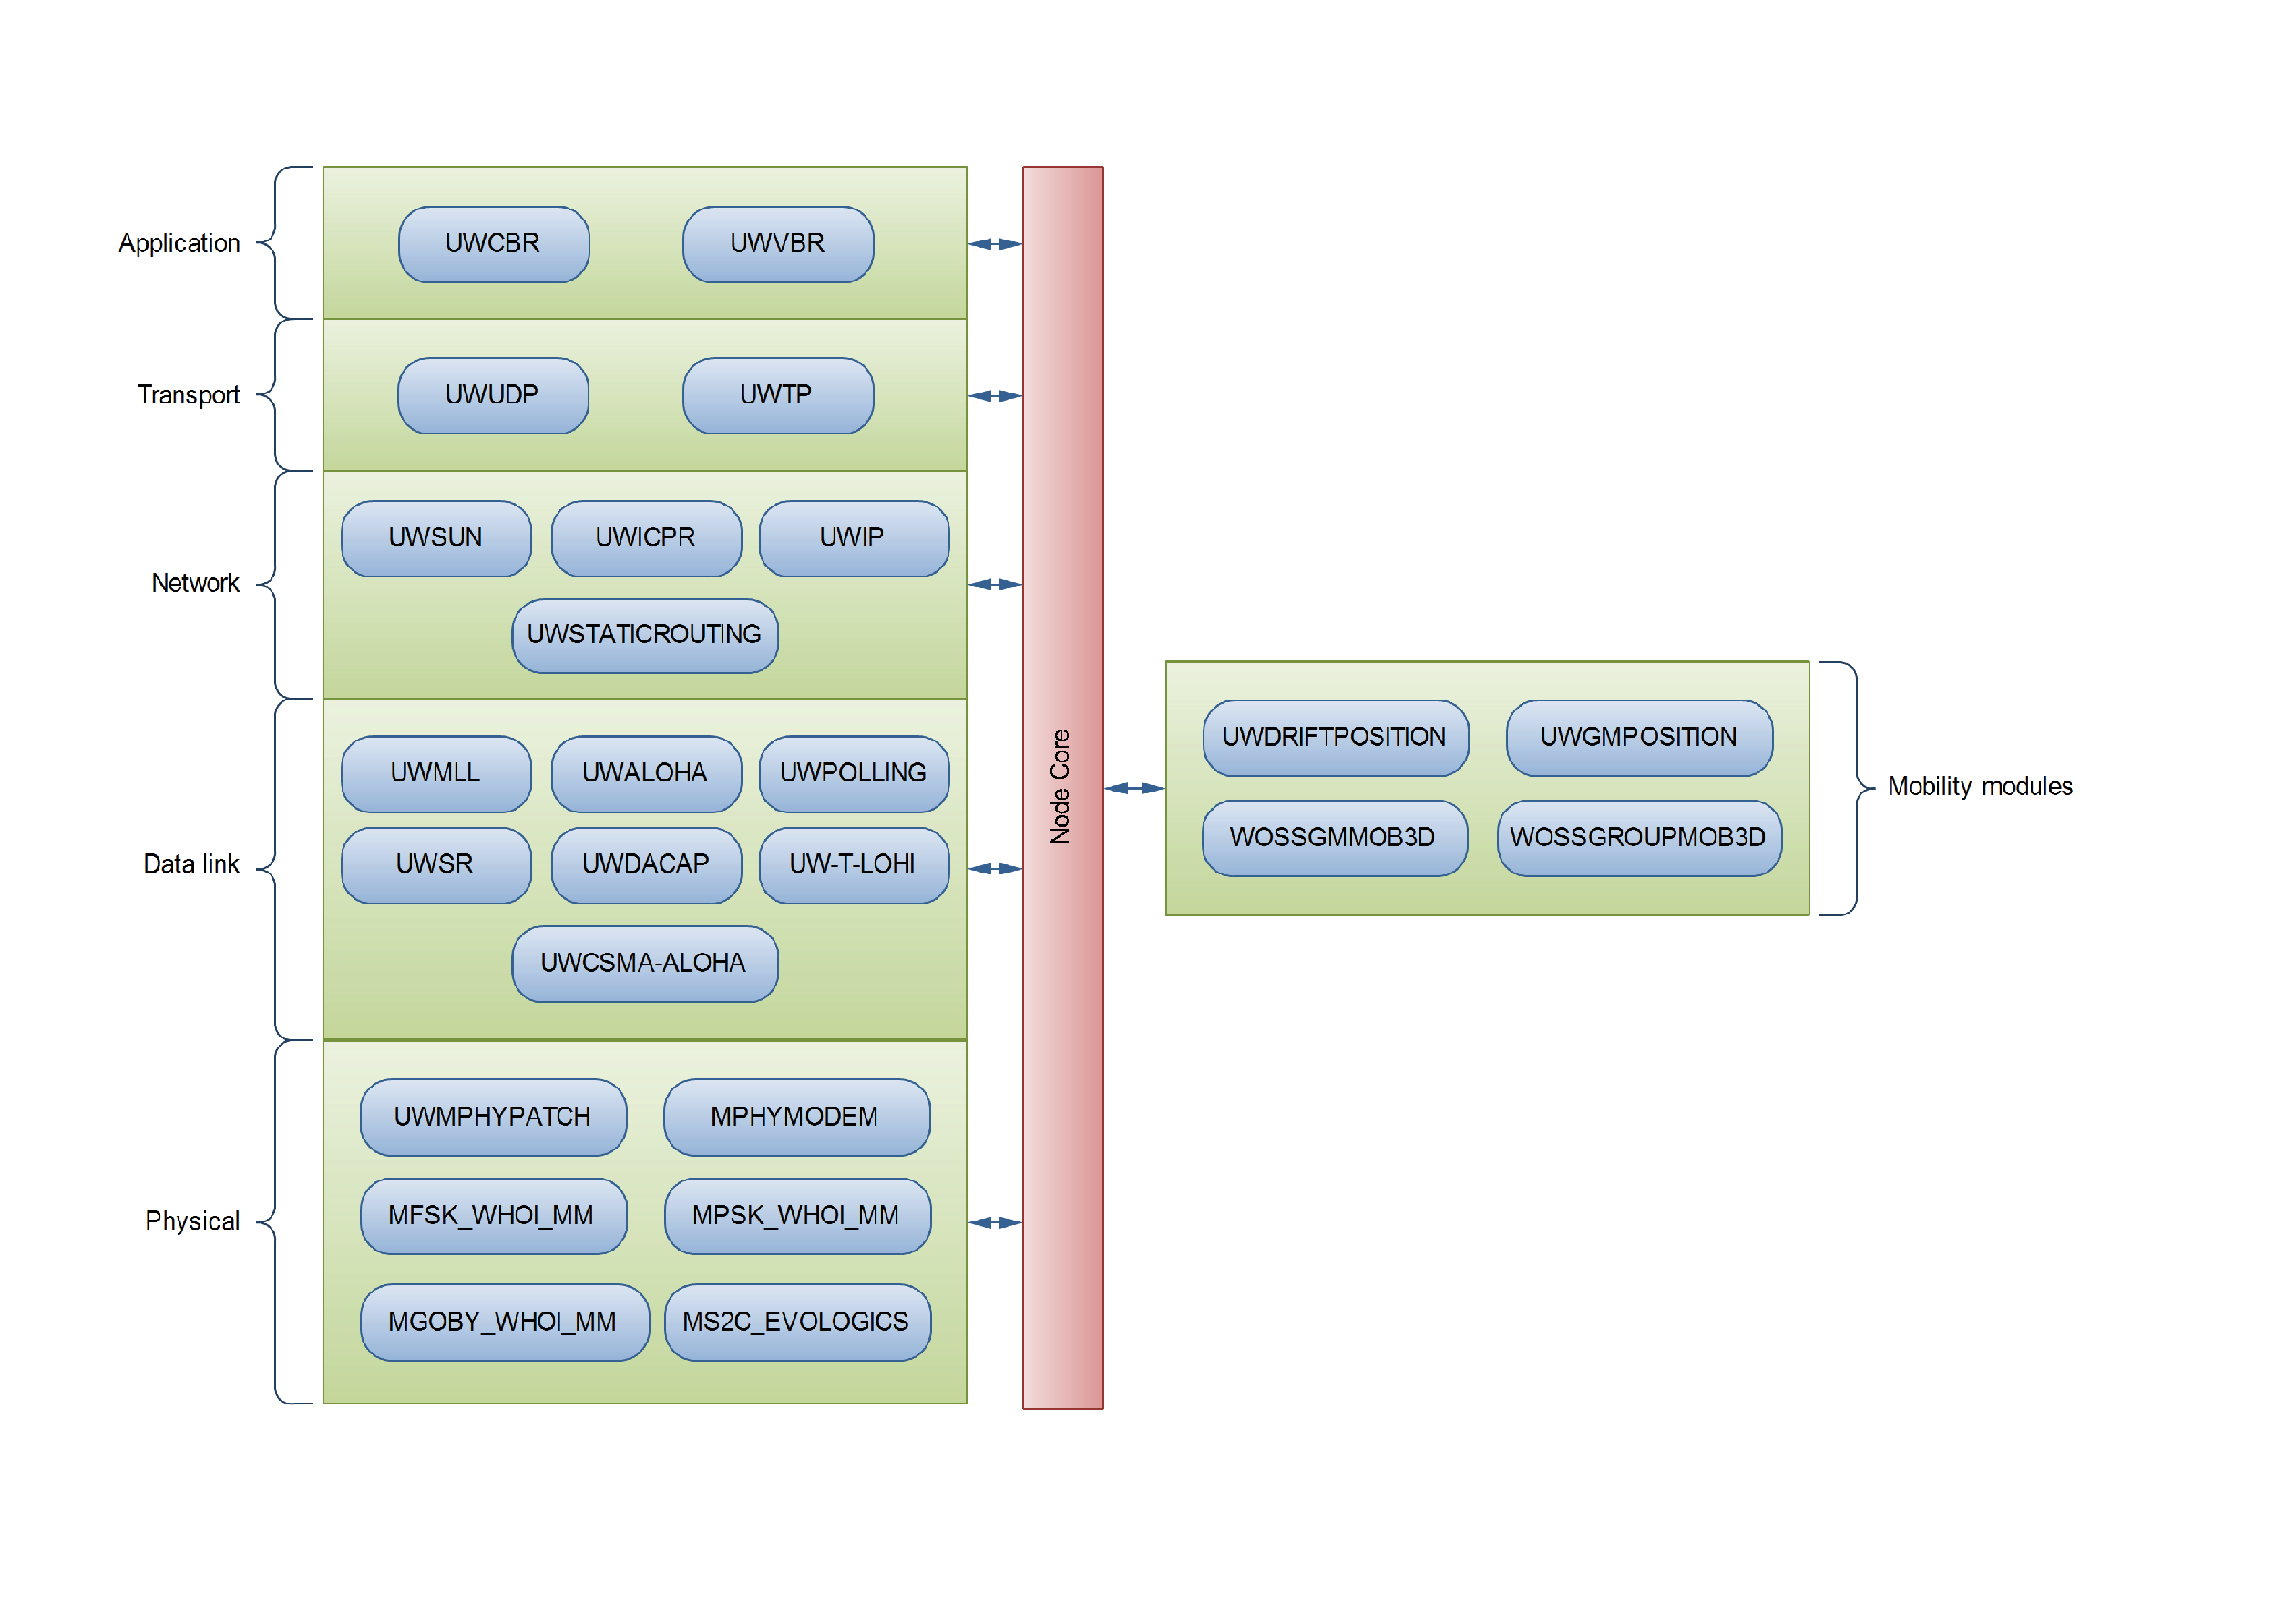
\includegraphics[width=\figw]{figure/DESERT_scheme.eps}
\centering 
\caption{Overview of the DESERT Underwater modules.}
\label{fig:scheme}
\end{center}
\end{figure}

\newpage


\section{Modules for the application layer}\label{sec:application}

\begin{description}
   \item {\bf Name:} {\tt uwcbr}
   \item {\bf Description:} This module implements a Constant Bit Rate (CBR) packet traffic between a sender and a receiver. The data traffic can be generated either by injecting packets in the network with a constant time period or according to a Poisson process with given mean. A single {\tt uwcbr} module represents a data flow between a pair of nodes: if there are two or more nodes transmitting to the same destination, the latter should have an equal number of {\tt uwcbr} modules, one for each flow. 
   \item {\bf Library name:} {\tt libuwcbr.so}
   \item {\bf Tcl name:} {\tt Module/UW/CBR}.
   \item {\bf Tcl parameters:} 
   \begin{description}
    \item {\tt period\_}: period between two consecutive packet transmissions;
    \item {\tt destPort\_}: {\tt Port} value of the destination;
    \item {\tt destAddr\_}: {\tt IP} of the destination;
    \item {\tt packetSize\_}: size of the packet payload;
    \item {\tt PoissonTraffic\_}: used to enable or disable the generation of traffic according to a Poisson distribution;
    \item {\tt debug\_}: flag to disable or enable debug messages [range in \{0,1\}] (optional, default value = 0);
    \item {\tt drop\_out\_of\_order\_}: flag used to change the behaviour of the module. If equals to 1 the module will accept packets only if in order, otherwise the module will accept them also out of order. (v1.1.0)
   \end{description}
   \item {\bf Tcl commands:}
   \begin{description}
    \item {\tt start}: start sending packets;
    \item {\tt stop}: stop sending packets;
    \item {\tt getrtt}: get the round trip time seen for the last received packet;
    \item {\tt getftt}: get the forward trip time;
    \item {\tt getper}: get the packet error rate;
    \item {\tt getthr}: get the throughput (in bytes/s);
    \item {\tt getrttstd}: get the standard deviation of the round trip time;
    \item {\tt getfttstd}: get the standard deviation of the forward trip time;
    \item {\tt getsentpkts}: get the number of {\tt CBR} packets sent;
    \item {\tt getrecvpkts}: get the number of {\tt CBR} packets received;
    \item {\tt getcbrheadersize}: get the size in byte of a {\tt hdr\_cbr} packet;
    \item {\tt sendPkt}: send a single {\tt CBR} packet;
    \item {\tt resetStats}: reset all the statistics;
   \end{description}
   \item {\bf Internal packet headers:} {\tt hdr\_uwcbr}.
   \item {\bf External packet headers:} {\tt hdr\_cmn} (common header from ns2); {\tt hdr\_uwip} (uwip header from DESERT);  {\tt hdr\_uwudp} (uwudp header from DESERT).
   \item {\bf Warnings:} This module requires an {\tt UWUDP} module below. A single {\tt UWCBR} module does not represent an application, but a single flow between two nodes: if there are two nodes transmitting to the same node, the latter should have two {\tt UWCBR modules}, one for each flow.
   \item {\bf Parent Libraries:}
   \begin{description}
   \item {\tt libMiracle.so}
   \item {\tt libuwip}
   \item {\tt libuwudp}
   \end{description}
   \item {\bf Tcl Scripts:} 
   \begin{description}
   \item {\tt samples/basic/uwcbr.tcl}
   \end{description}
\end{description}

\vspace{1 cm}

\begin{description}
    \item {\bf Name:} {\tt uwvbr}
    \item {\bf Description:} This module implements a Variable Bit Rate (VBR) packet traffic between a sender and a receiver. The data packet generation process takes place by switching between two different CBR processes, e.g., having different average packet inter-arrival times. 
    The switch between the processes can be configured by the user by providing the switching epochs. Otherwise, the simulator can be instructed to switch at constant or exponentially distributed intervals. A single {\tt uwvbr} module represents a data flow between a pair of nodes: if there are two or more nodes transmitting to the same node, the latter should have an equal number of {\tt uwvbr} modules, one for each flow.
   \item {\bf Library name:} {\tt libuwvbr.so}
   \item {\bf Tcl parameters:} 
   \begin{description}
    \item {\tt period\_}: period between two consecutive packet transmissions;
    \item {\tt destPort\_}: {\tt Port} value of the destination;
    \item {\tt destAddr\_}: {\tt IP} of the destination;
    \item {\tt packetSize\_}: size of the packet payload;
    \item {\tt PoissonTraffic\_}: flag used to enable or disable the generation of traffic according to a Poisson distribution;
    \item {\tt debug\_}: flag to disable or enable debug messages [range in \{0,1\}] (optional, default value = 0);
    \item {\tt drop\_out\_of\_order\_}: flag used to change the behaviour of the module. If equals to 1 the module will accept packets only if in order, otherwise the module will accept them also out of order. (v1.1.0)
   \end{description}
   \item {\bf Tcl commands:}
   \begin{description}
    \item {\tt start}: start sending packets;
    \item {\tt stop}: stop sending packets;
    \item {\tt getrtt}: get the round trip time seen for last received packet;
    \item {\tt getftt}: get the forward trip time;
    \item {\tt getper}: get the packet error rate;
    \item {\tt getthr}: get the throughput (in bytes/s);
    \item {\tt getrttstd}: get the standard deviation of the round trip time;
    \item {\tt getfttstd}: get the standard deviation of the forward trip time;
    \item {\tt getsentpkts}: get the number of {\tt VBR} packets sent;
    \item {\tt getrecvpkts}: get the number of {\tt VBR} packets received;
    \item {\tt getvbrheadersize}: return the size in byte of a {\tt hdr\_vbr} packet;
    \item {\tt sendPkt}: send a single {\tt VBR} packet;
    \item {\tt resetStats}: reset all the statistics;
   \end{description}
   \item {\bf Internal packet headers:} {\tt hdr\_uwvbr}.
   \item {\bf External packet headers:} {\tt hdr\_cmn} (common header from ns2); {\tt hdr\_uwip} (uwip header from DESERT);  {\tt hdr\_uwudp} (uwudp header from DESERT).
   \item {\bf Warnings:} This module requires an {\tt UWUDP} module below. A single {\tt UWVBR} module does not represent an application, but a single flow between two nodes: if there are two nodes transmitting to the same node, the latter should have two {\tt UWVBR modules}, one for each flow.
   \item {\bf Parent Libraries:}
   \begin{description}
   \item {\tt libMiracle.so}
   \item {\tt libuwip}
   \item {\tt libuwudp}
   \end{description}
   \item {\bf Tcl Scripts:} 
   \begin{description}
   \item {\tt samples/basic/uwvbr.tcl}
   \end{description}
\end{description} 

\section{Modules for the transport layer}\label{sec:transport}

\begin{description}
   \item {\bf Name:} {\tt uwudp}
   \item {\bf Description:} This module implements the flow multiplexing and demultiplexing from and to the upper layers, respectively.  It does not support link reliability, error detection or flow control.
   \item {\bf Library name:} {\tt libuwudp.so}
   \item {\bf Tcl name:} {\tt Module/UW/UDP}
   \item {\bf Tcl parameters:}
    \begin{description}
     \item {\tt debug\_}: flag to disable or enable debug messages [range in \{0,1\}] (optional, default value = 0).
    \end{description}
   \item {\bf Tcl commands:}
    \begin{description}
   	 \item {\tt getudpheadersize}: get the size of the {\tt UDP} packet header;
   	 \item {\tt assignPort}: create an association between the {\tt UDP} module and an upper module (example: {\tt \$udp(\$id) assignPort \$cbr(\$id)}).
 	\end{description}
   \item {\bf Internal packet headers:} {\tt hdr\_uwudp}.
   \item {\bf External packet headers:} {\tt hdr\_cmn} (common header from ns2); {\tt hdr\_uwip} (uwip header from DESERT).
   \item {\bf Warnings:} none.
   \item {\bf Parent Libraries:}
   \begin{description}
   \item {\tt libuwip}
   \end{description}
   \item {\bf Tcl Scripts:} 
   \begin{description}
   \item {\tt samples/basic/uwvbr.tcl}
   \end{description}
\end{description}

\vspace{1 cm}

\begin{description}
   \item {\bf Name:} {\tt uwtp}
   \item {\bf Description:} As the previous {\tt uwudp}, this transport layer module handles the multiplexing and de-multiplexing of data    	flows, but it also supports an error control technique, as well as in-order data delivery to the upper layers. In more detail, {\tt uwtp} includes an Automatic Repeat reQuest (ARQ) error control technique.  This module can handle both ACK and NACK messages, as well as cumulative ACKs. To work correctly, {\tt uwtp} has to know the destination port number of each application flow it handles: this information must be provided during the setting of the parameters for the simulations or tests that have to be conducted.
   \item {\bf Library name:} {\tt libuwtp.so}
   \item {\bf Tcl name:} {\tt Module/UW/TP}
   \item {\bf Tcl parameters:} 
    \begin{description}
      \item{\tt debug\_}: flag to disable or enable debug messages [range in \{0,1\}] (optional, default value = 0).
      \item{\tt send\_buffer\_size\_}: size of the sender buffer. 
      \item{\tt receive\_buffer\_size\_}: size of the receiver buffer.
      \item{\tt delay\_interval\_}: the maximum delay time to be considered before transmitting a NACK packet.
      \item{\tt destPort\_}: destination port number.
      \item{\tt nack\_retx\_time\_}: timer for NACK retransmission. When this timer expires, the receiver is forced to send a given NACK packet again.
      \item{\tt pkt\_delete\_time\_from\_queue\_}: timer to delete packets from the transmission queue (e.g., when the acknowledgement mechanism is not enabled or when an ACK packet is lost).
      \item{\tt expected\_ACK\_threshold\_}: threshold used to tune the number of generated ACK packets when the cumulative ACK mode is on.\end{description}
   \item {\bf Tcl commands:}
    \begin{description}
      \item{\tt getUWTPDataHSize}: get the size of data packet header in Bytes;
      \item{\tt getUWTPAckHSize}: get the size of the ACK packet header in Bytes; 
      \item{\tt getUWTPNackHSize}: get the size of the NACK packet header in Bytes;
      \item{\tt getAckTxCount}: get the number of ACK packets transmitted by a node throughout the communication;
      \item{\tt getNackTxCount}: get the number of NACK packets transmitted by a node throughout the communication;
      \item{\tt getAckRxCount}: get the number of ACK packets received by a node throughout the communication;
      \item{\tt getNackRxCount}: get the number of NACK packets received by a node throughout the communication;
      \item{\tt setAckMode}: set the protocol to function with ARQ techniques;
      \item{\tt setNoAckMode}: set the protocol to function without ARQ techniques (only packet buffering is performed);
      \item{\tt setCumAckMode}: if ACK mode is set, then use the cumulative ACK technique;
      \item{\tt setNoCumAckMode}: if ACK mode is set, then do not use the cumulative ACK technique.
    \end{description}
   \item {\bf Internal packet headers:} {\tt hdr\_uwtp}, {\tt hdr\_uwtp\_data}, {\tt hdr\_uwtp\_ack}, and {\tt hdr\_uwtp\_nack}.
   \item {\bf External packet headers:} {\tt hdr\_cmn} (common header from ns2); {\tt hdr\_uwip} (uwip header from DESERT).
   \item {\bf Warnings:} This module requires to pass the destination port number from TCL script (for instance, {\tt set destPort\_ \$destination\_port\_number}).
   \item {\bf Parent Libraries:}
   \begin{description}
   \item {\tt libuwip}
   \end{description}
   \item {\bf Tcl Scripts:} 
   \begin{description}
   \item {\tt Not provided with DESERT v 1.0.0.}
   \end{description}
\end{description}


\section{Modules for the network layer}\label{sec:network}

\begin{description}
   \item {\bf Name:} {\tt uwstaticrouting}
   \item {\bf Description:} This module makes it possible to simulate and test data traffic which has to follow predetermined routes. For each network node, there is an option to choose a default gateway and/or fill a static routing table (whose maximum size is hard-coded and fixed to $100$ entries). This information is then exploited locally at each node to forward the network packets, hop by hop, throughout the predetermined paths.
   \item {\bf Library name:} {\tt libuwstaticrouting.so}
   \item {\bf Tcl name:} {\tt Module/UW/StaticRouting}.
   \item {\bf Tcl parameters:} none.
   \item {\bf Tcl commands:}
   	\begin{description}
   	 \item {\tt numroutes}: return the size of the routing table;
   	 \item {\tt clearroutes}: clear all the routing table information;
 	 \item {\tt printroutes}: print the routing table;
 	 \item {\tt defaultGateway}: set the {\tt IP} address of the {\tt default gateway} (example {\tt \$ipr(1) defaultGateway "1.0.0.254"});
 	 \item {\tt addroute}: add an entry in the routing table (example {\tt \$ipr(1) addRoute "1.0.0.1" "1.0.0.2"}, where the first {\tt IP} address is the destination, the second one is the next hop);
 	\end{description}
   \item {\bf Internal packet headers:} none.
   \item {\bf External packet headers:} {\tt hdr\_cmn} (common header from ns2); {\tt hdr\_uwip} (uwip header from DESERT).
   \item {\bf Warnings:} The maximum size of the routing table is hard-coded, the name of the corresponding variable is {\tt IP\_ROUTING\_MAX\_ROUTES} and its value is fixed to 100.
   \item {\bf Parent Libraries:}
   \begin{description}
   \item {\tt libMiracle.so}
   \item {\tt libuwip}
   \end{description}
   \item {\bf Tcl Scripts:} 
   \begin{description}
   \item {\tt samples/basic/uwvbr.tcl.}
   \end{description}
\end{description}

\vspace{1 cm}

\begin{description}
   \item {\bf Name:} {\tt uwsun}
   \item {\bf Description:} This module implements a dynamic, reactive source routing protocol. The generation of routing paths can be made based on different criteria, such as the minimization of the hop-count or the maximization of the minimum Signal to Noise Ratio (SNR) along the links of the path. {\tt uwsun} is also designed to collect and process different statistics of interest for the routing level. Currently, this module supports all application modules provided in DESERT (i.e., {\tt uwcbr} and {\tt uwvbr}), and it can be easily extended. 
   \item {\bf Library name:} {\tt libuwsun.so}
   \item {\bf Tcl name:} {\tt Module/UW/SUNNode} for the nodes, {\tt Moudle/UW/SUNSink} for the sinks.
   \item {\bf Tcl parameters (Node):}
   \begin{description}
   	 \item {\tt ipAddr\_}: {\tt IP} of the node;
   	 \item {\tt subnet\_}: subnet mask of the node; (removed in v1.0.1)
 	 \item {\tt metrics\_}: metric used by the node during routing;
 	 \item {\tt PoissonTraffic\_}: flag used to enable or disable the generation of traffic according to a Poisson distribution;
 	 \item {\tt period\_status\_}: period of the Poisson distribution for the status packets;
 	 \item {\tt period\_data\_}: period of the Poisson distribution for the data packets;
 	 \item {\tt setAckMode\_}: flag to enable or disable the ARQ mechanism (NOTE: in order to completely disable the ARQ mechanism you have also to set the {\tt max\_ack\_error\_} parameter to 1); (removed in v1.0.1)
 	 \item {\tt max\_ack\_error\_}: maximum number of retransmission for the ARQ;
 	 \item {\tt timer\_route\_validity\_}: timer to determine the maximum time duration (in seconds) during which to consider valid a route established between a node and a sink;
 	 \item {\tt timer\_ack\_waiting\_}: timer to determine the maximum waiting time (in seconds) for an ACK (this value depends on both the observed sound speed profile and the distance between sender and transmitter);
 	 \item {\tt timer\_sink\_probe\_validity\_}: timer to determine the maximum time duration (in seconds) during which to consider valid a probe received from a sink;
 	 \item {\tt timer\_buffer\_}: timer to determine the time (in seconds) between two buffer processes; 	 
 	 \item {\tt printDebug\_}: flag used to print debug information; 	 
 	 \item {\tt probe\_min\_snr\_}: SNR threshold to consider valid the probe received from a sink (i.e., the SNR of the received probe must be above this threshold to be considered valid); 	 
 	 \item {\tt buffer\_max\_size\_}: the maximum size of the buffer;
 	 \item {\tt safe\_timer\_buffer\_}: flag used to enable several mechanisms that adapt the timer\_buffer\_ value automatically; (from v 1.1.0)
 	 \item {\tt disable\_path\_error\_}: used to disable the error messages. (from v 1.1.1)
 	\end{description}
   \item {\bf Tcl parameters (Sink):}
    \begin{description}
     \item {\tt ipAddr\_}: {\tt IP} of the node;
   	 \item {\tt subnet\_}: subnet mask of the node; (removed in v1.0.1)
   	 \item {\tt setAckMode\_}: flag to enable or disable the ARQ mechanism; (removed in v1.0.1)
   	 \item {\tt t\_probe}: time (in seconds) between two successive sink probes;
   	 \item {\tt PoissonTraffic\_}: flag used to enable or disable the generation of traffic according to a Poisson distribution;
   	 \item {\tt periodPoissonTraffic\_}: period of the Poisson distribution for the status packets;
     \item {\tt printDebug\_}: flag used to print debug information; 	  
    \end{description}
   \item {\bf Tcl commands (Node):} 
    \begin{description}
    \item {\tt initialize}: retrieve the {\tt IP} address from the {\tt IP} module (NOTE: this command is mandatory, and it must be used after the assignment of the {\tt IP} address to the node);
    \item {\tt printhopcount}: print the number of hops needed by the node to reach the sink;
    \item {\tt printhops}: print the routing table of the node;
    \item {\tt getackcount}: get the number of {\tt hdr\_sun\_ack} packets generated by all the nodes;
    \item {\tt getdatapktcount}: get the number of {\tt hdr\_sun\_data} packets received from the upper layers by the entire network;
    \item {\tt getforwardedcount}: get the number of {\tt hdr\_sun\_data} packets forwarded by the entire network;
    \item {\tt getdatapktdroppedbuffer}: get the number of {\tt hdr\_sun\_data} packets dropped by the entire network because the buffer was full;
    \item {\tt getdatapktdroppedmaxretx}: get the number of {\tt hdr\_sun\_data} packets dropped by the entire network because the maximum number of retransmission has been reached;
    \item {\tt getpathestablishmentpktcount}: get the number of {\tt hdr\_sun\_path\_est} packets generated by the entire network;
    \item {\tt getackheadersize}: get the size in Bytes of a {\tt hdr\_sun\_ack} packet;
    \item {\tt getdatapktheadersize}: get the size in Bytes of a {\tt hdr\_sun\_data} packet;
    \item {\tt getpathestheadersize}: get the size in Bytes of a {\tt hdr\_sun\_path\_est} packet;
    \item {\tt getstats}: get the number of packets sent by a node with a specific hop count value (example: {\tt set stat\_ [\$ipr(\$i) getstats \$j]}, where \$j is the hop count value);
    \item {\tt trace}: used to set the file name of the trace file in which UWSUN will save information about the packets processed.
    \end{description}
   \item {\bf Tcl commands (Sink):} 
    \begin{description}
    \item {\tt initialize}: retrieve the {\tt IP} address of the node from the {\tt IP} module (NOTE: this command is mandatory, and it must be used, in the tcl configuration script, after the assignment of the {\tt IP} address to the node);
    \item {\tt start}: start to send probe messages;
    \item {\tt stop}: stop to send probe messages;
    \item {\tt sendprobe}: send a single probe message;
    \item {\tt getprobetimer}: get the timer of the probe messages;
    \item {\tt getprobepktcount}: get the number of {\tt hdr\_sun\_probe} packets generated by the sinks;
    \item {\tt getackcount}: get the number of {\tt hdr\_sun\_ack} packets generated by the sinks;
    \item {\tt getprobepktheadersize}: get the size in Bytes of a {\tt hdr\_sun\_probe} packet;  
    \item {\tt getackheadersize}: get the size in Bytes of a {\tt hdr\_sun\_ack} packet;
    \item {\tt setnumberofnodes}: set the number of nodes in the simulation (NOTE: do not count the sinks!). This value is used to compute and save statistics (example: {\tt \$ipr\_sink setnumberofnodes \$opt(nn)};
    \item {\tt getstats}: get the number of packets received by the sink from a specific node with a specific hop count value (example: {\tt set stats(\$j) [\$ipr\_sink getstats \$i \$j]}, where {\tt \$i} is the last Byte of the {\tt IP} of the node, and {\tt \$j} is the hop count value);
    \item {\tt trace}: used to set the file name of the trace file in which UWSUN will save information about the packets processed.
    \end{description} 
   \item {\bf Internal packet headers:} {\tt hdr\_sun\_ack}; {\tt hdr\_sun\_data}; {\tt hdr\_sun\_path\_est}; {\tt hdr\_sun\_probe}.
   \item {\bf External packet headers:} {\tt hdr\_cmn} (common header from ns2); {\tt hdr\_uwcbr} (uwcbr header from DESERT); {\tt hdr\_uwip} (uwip header from DESERT); {\tt hdr\_MPhy} (MPhy header from ns-miracle)
   \item {\bf Warnings:} The call to the {\tt initialize} command is mandatory for both sinks and nodes (it is possible to avoid it only by setting manually the {\tt ipAddr\_}). In order to notify the presence of the sink it is mandatory to send at least one probe with the command {\tt sendprobe}, or periodically with {\tt start}. If you want to disable completely the {\tt ARQ} you have to: set to 1 {\tt buffer\_max\_size\_} and {\tt max\_ack\_error\_}, and to 0 {\tt setAckMode\_} for both sinks and nodes. The maximum number of hops that a packet can perform is hard-coded and tuned to avoid flooding and increase performance (it is however possible to change such value by modifying the field {\tt MAX\_HOP\_NUMBER} in the source file {\tt sun-ipr-common-structures.h}).
   \item {\bf Parent Libraries:}
   \begin{description}
      \item {\tt libMiracle.so}
      \item {\tt libmphy}
      \item {\tt libuwip}
      \item {\tt libuwcbr}
   \end{description}
   \item {\bf Tcl Scripts:} 
   \begin{description}
      \item {\tt samples/basic/uwsun.tcl}
   \end{description} 
\end{description}

\vspace{1 cm}

\begin{description}
   \item {\bf Name:} {\tt uwicrp}
   \item {\bf Description:} This module, which requires very few configuration parameters, implements a simple flooding-based routing mechanism called Information-Carrying Based Routing protocol, see~\cite{LiangTakamatsu}.
   \item {\bf Library name:} {\tt libuwicrp.so}
   \item {\bf Tcl name:} {\tt Module/UW/ICRPNode} for the nodes; {\tt Moudle/UW/ICRPSink} for the sinks.
   \item {\bf Tcl parameters (Node):}
   \begin{description}
    \item {\tt ipAddr\_}: {\tt IP} of the node;
    \item {\tt printDebug\_}: flag to print debug information;
    \item {\tt maxvaliditytime\_}: the maximum validity period for a route established between a node and a sink;
    \item {\tt timer\_ack\_waiting\_}: timer to determine the maximum waiting time (in seconds) for an ACK (this value depends on both the observed sound speed profile and the distance between sender and transmitter);
   \end{description}
   \item {\bf Tcl parameters (Sink):}
   \begin{description}
    \item {\tt ipAddr\_}: {\tt IP} of the sink;
    \item {\tt printDebug\_}: flag to print debug information;
   \end{description}
   \item {\bf Tcl commands (Node):}
   \begin{description}
    \item {\tt initialize}: retrieve the {\tt IP} address of the node from the {\tt IP} module (NOTE: this command is mandatory, and it must be used, in the tcl configuration script, after the assignment of the {\tt IP} address to the node);
    \item {\tt printhops}: print the routing table of the node;
    \item {\tt clearhops}: clear all the routing information;
    \item {\tt getackheadersize}: get the size in Bytes of a {\tt hdr\_uwicrp\_ack} packet;
    \item {\tt getdataheadersize}: get the size in Bytes of a {\tt hdr\_uwicrp\_data} packet;
    \item {\tt getstatusheadersize}: get the size in Bytes of a {\tt hdr\_uwicrp\_status} packet;
    \item {\tt getackcount}: get the number of {\tt hdr\_uwicrp\_ack} packets generated by the nodes;
    \item {\tt getdatapktcount}: get the number of {\tt hdr\_uwicrp\_data} packets generated by all the nodes;
    \item {\tt getstatuspktcount}: get the number of {\tt hdr\_uwicrp\_status} packets forwarded by all the nodes;
    \item {\tt ipsink}: notify to the node the {\tt IP} address of the sink (example: {\tt \$ipr ipsink "1.0.0.254"}).
   \end{description}
   \item {\bf Tcl commands (Sink):}
   \begin{description}
    \item {\tt initialize}: retrieve the {\tt IP} address of the node from the {\tt IP} module (NOTE: this command is mandatory, and it must be used, in the tcl configuration script, after the assignment of the {\tt IP} address to the node);
    \item {\tt getackheadersize}: get the size in Bytes of a {\tt hdr\_uwicrp\_ack} packet;
    \item {\tt getdataheadersize}: get the size in Bytes of a {\tt hdr\_uwicrp\_data} packet;
    \item {\tt getstatusheadersize}: get the size in Bytes of a {\tt hdr\_uwicrp\_status} packet;
    \item {\tt getackcount}: get the number of {\tt hdr\_uwicrp\_ack} packets generated by the sink;
    \item {\tt getstatuspktcount}: get the number of {\tt hdr\_uwicrp\_status} packets generated by the sinks.
   \end{description}
   \item {\bf Internal packet headers:} {\tt hdr\_uwicrp\_ack}; {\tt hdr\_uwicrp\_data}; \\ {\tt hdr\_uwicrp\_status}.
   \item {\bf External packet headers:} {\tt hdr\_cmn} (common header from ns2); {\tt hdr\_uwip} (uwip header from DESERT).
   \item {\bf Warnings:} The call to the {\tt initialize} command is mandatory for both sinks and nodes (it is possible to avoid it only by setting manually the {\tt ipAddr\_}). For the nodes it is also mandatory to set manually the {\tt IP} of the sink using the command {\tt ipsink}. The maximum number of hops that a packet can perform is hard-coded and tuned to avoid flooding and increase performance (it is however possible to change such value by modifying the field {\tt MAX\_HOP\_NUMBER} in the source file {\tt uwicrp-common.h}).
   \item {\bf Parent Libraries:}
    \begin{description}
     \item {\tt libMiracle.so}
     \item {\tt libuwip}
    \end{description}
   \item {\bf Tcl Scripts:} 
    \begin{description}
     \item {\tt samples/basic/uwicrp.tcl}
    \end{description}
\end{description}

\vspace{1 cm}

\begin{description}
   \item {\bf Name:} {\tt uwip}
   \item {\bf Description:} This module is used to assign an address to the nodes in a given network according to the standard IPv4 addresses; it provides the Time-To-Live (TTL) functionality and does not implement any routing mechanism. It can be configured to provide all the functional and procedural means intended for an Internet Protocol module (e.g., fragmentation, data reassembly and notification of delivery errors).
   \item {\bf Library name:} {\tt libuwip.so}
   \item {\bf Tcl name:} {\tt Module/UW/IP}
   \item {\bf Tcl parameters:}
    \begin{description}
     \item {\tt debug\_}: flag to disable or enable debug messages [range in \{0,1\}] (optional, default value = 0).
    \end{description}
   \item {\bf Tcl commands:}
    \begin{description}
     \item {\tt setaddrinet}: it is used to set the address type of the packets to {\tt NS\_AF\_INET}. See {\tt UWMLL} module for more information;
     \item {\tt setaddrilink}: it is used to set the address type of the packets to {\tt NS\_AF\_ILINK}. See {\tt UWMLL} module for more information;
     \item {\tt addr-string} return the {\tt IP} address of the node in the standard form (e.g., {\tt 1.0.0.2});
     \item {\tt getipheadersize}: get the size in Bytes of a {\tt hdr\_uwip} packet;
     \item {\tt addr}: set the {\tt IP} of a given node (example {\tt \$ip addr "1.0.0.1"});
    \end{description}
   \item {\bf Internal packet headers:} {\tt hdr\_uwip}.
   \item {\bf External packet headers:} {\tt hdr\_cmn} (common header from ns2).
   \item {\bf Warnings:} It is possible to obtain the {\tt IP} address from an {\tt UWIP} module with a synchronous message called {\tt UWIPClMsgReqAddr}.
   \item {\bf Parent Libraries:} {\tt libMiracle.so}
   \item {\bf Tcl Scripts:} 
   \begin{description}
   \item {\tt samples/basic/uwcbr.tcl}.
   \end{description}
\end{description}

\section{Modules for the data link layer}\label{sec:data_link}

\begin{description}
   \item {\bf Name:} {\tt uwmll}
   \item {\bf Description:} Since node-to-node communications at the link layer are performed using MAC addresses whereas the communications at the upper layers employ IP addresses, a method to associate the latter to the former is required.
   With {\tt uwmll}, it is possible to set the correspondence between IP and MAC addresses a priori, by filling an ARP table for each network node. Alternatively, ARP tables can be automatically filled using the Address Resolution Protocol (ARP). The {\tt uwmll} module must be placed between one (or more) IP module(s) and one MAC module.
   \item {\bf Library name:} {\tt libuwmll.so}
   \item {\bf Tcl name:} {\tt Module/UW/MLL}
   \item {\bf Tcl parameters:} none
   \item {\bf Tcl commands:} 
    \begin{description}
     \item{\tt reset} : reset the table entries (i.e., clear the ARP table).
     \item{\tt addentry} : associate IP and MAC addresses in the ARP table (example: {\tt  addentry [\$ip\_ addr] [\$mac\_ addr]}, where {\tt [\$ip\_ addr]} and {\tt [\$ip\_ addr]} return the addresses of given {\tt IP} and {\tt MAC} modules, respectively). This command helps to reduce the overhead of resolving IP addresses in the whole network. 
    \end{description}
   \item {\bf Internal packet headers:} {\tt hdr\_mac} (mac header from ns-miracle)
   \item {\bf External packet headers:} {\tt hdr\_cmn} (common header from ns2) and  {\tt hdr\_uwip} (IP header from DESERT)
   \item {\bf Warnings:} whilst this module appears to work properly in 64 bit OS, we experienced problems with some Tcl scripts in 32 bit OS. We are currently working to identify and solve the corresponding bugs. Please, contact our research team for more information.
NOTE: alternatively to this module, it may be used the {\tt mll} module already included in NS-Miracle.
   \item {\bf Parent Libraries:}
       \begin{description}
         \item {\tt libMiracle.so}
	      \item {\tt libmphy.so} 
	      \item {\tt libmmac.so}
        \end{description}
   \item {\bf Tcl Scripts:}  All the tcl samples provided with DESERT Underwater v1.0.0 use MLL layer. In each tcl sample you can see how MLL works.
\end{description}

\vspace{1 cm}

\begin{description}
   \item {\bf Name:} {\tt uwaloha}
   \item {\bf Description:} ALOHA is a random access scheme, i.e., a protocol that allows nodes to send data packets directly without any preliminary channel reservation process. In its original version~\cite{Abramson85}, neither channel sensing nor retransmission is implemented and each node can transmit whenever it has data packets to send. As a consequence, packet losses can occur. In later adaptations~\cite{GuoSingapore}, ALOHA has been enhanced with acknowledgment packets (ALOHA-ACK). The {\tt uwaloha} module implements the functionality of the basic ALOHA protocol as well as its enhanced version using ARQ for error control. It is possible to freely switch between basic ALOHA and ALOHA-ACK.
   \item {\bf Library name:} {\tt libuwaloha.so} 
   \item {\bf Tcl name:} {\tt Module/UW/ALOHA}
   \item {\bf Tcl parameters:} 
    \begin{description}
     \item {\tt HDR\_size\_} : size of the packet header (to be used if there is any internal packet header);
     \item {\tt ACK\_size\_} : size of the ACK packet (if the ARQ technique is enabled);
     \item {\tt max\_tx\_tries\_} : maximum number of retransmission attempts;
     \item {\tt wait\_constant\_} : time interval guard to handle the arrival of ACK packets according to different delays;
     \item {\tt uwaloha\_debug\_} : flag to enable debug messages if set to any value different than $0$;
     \item {\tt max\_payload\_} : maximum number of payload in a packet;
     \item {\tt ACK\_timeout\_} : initialization value for the ACK timeout;
     \item {\tt alpha\_} : smoothing factor variable used to compute the Round Trip Time (RTT);
     \item {\tt buffer\_pkts\_} : maximum number of packets that can be stored in the buffer;
     \item {\tt backoff\_tuner\_} : duration of the backoff period;
     \item {\tt max\_backoff\_counter\_} : maximum number of backoff re-computations (the backoff is increased exponentially).
    \end{description}(i.e., plain ALOHA);
     \item {\tt initialize} : initialize the necessary parameters of the protocol;
     \item {\tt setAckMode} : enable the ARQ technique (i.e., ALOHA-ARQ);
     \item {\tt setNoAckMode} : disable the ARQ technique (i.e., plain ALOHA); 
     \item {\tt printTransitions} : print the information about the protocol state machine transitions into a file;	
     \item {\tt getQueueSize} : get the number of buffered packets;
     \item {\tt setMacAddr:} set the MAC address of the node (NOTE: this value is an integer value and should be different for every node in the network. If this command is not used, the node will have a default MAC address computed according to counting variable in the corresponding base class). 
      \item {\bf Internal packet headers:} none
      \item {\bf External packet headers:} {hdr\_cmn} (common header from ns2) and {\tt hdr\_mac} (MAC header from ns-miracle)
      \item {\bf Warnings:} none
      \item {\bf Parent Libraries:} 
        \begin{description}
         \item {\tt libMiracle.so}
	      \item {\tt libmphy.so} 
	      \item {\tt libmmac.so}
        \end{description}
   \item {\bf Tcl Scripts:}
      \begin{description}
	    \item {\tt samples/basic/test\_uw\_aloha\_simple.tcl}
	    \item {\tt samples/advanced/test\_uw\_aloha.tcl}
      \end{description}
\end{description}

\vspace{1 cm}

\begin{description}
   \item {\bf Name:} {\tt uwsr}
   \item {\bf Description:} Automatic Repeat reQuest (ARQ) is the basic mechanism to ensure that no erroneous packets are delivered to layers higher than the data-link. When a packet is received with errors, the receiver may ask for retransmissions by sending a small packet called NACK (Negative ACKnowledgment). Similarly, a successful transmission can be notified to the transmitter via an ACK packet. Selective Repeat ARQ allows the transmitter to send up to N consecutive packets before waiting for ACKs or NACKs. The packets sent and not yet acknowledged must be buffered by the transmitter; the receiver can also buffer packets and, in case of errors, only the erroneous packets are sent again. {\tt uwsr} implements a Selective Repeat ARQ mechanism in combination with an Additive Increase and Multiplicative Decrease (AIMD) congestion control technique, similar to TCP's congestion window size adaptation. This protocol has been shown to be effective because the underwater channel propagation delay is sufficiently large to accommodate more than one packet transmission within one round-trip time (RTT)~\cite{AzadSantander}. 
   \item {\bf Library name:} {\tt libuwsr.so}
   \item {\bf Tcl name:} {\tt Module/UW/USR}
   \item {\bf Tcl parameters:} 
    \begin{description}
     \item {\tt HDR\_size\_} : size of the packet header (if applicable);
     \item {\tt ACK\_size\_} : size of the ACK packet (if the ARQ technique is enabled);
     \item {\tt max\_tx\_tries\_} : maximum number of retransmission attempts;
     \item {\tt wait\_constant\_} : time interval guard to handle the arrival of ACK packets according to different delays;
     \item {\tt uwsr\_debug\_} : flag to enable debug messages if set to any value different than $0$;
     \item {\tt max\_payload\_} : maximum payload size in a DATA packet;
     \item {\tt ACK\_timeout\_} : initialization value for the ACK timeout [s];
     \item {\tt alpha\_} : smoothing factor variable used to compute the Round Trip Time (RTT);
     \item {\tt buffer\_pkts\_} : maximum number of packets that can be stored in the buffer;
     \item {\tt backoff\_tuner\_:} multiplying factor used in the calculation of the backoff timer;   
     \item {\tt max\_backoff\_counter\_} : maximum number of times a backoff timer can be called (the backoff is increased exponentially);
     \item {\tt listen\_time\_:} duration [s] of the channel sensing period;
     \item {\tt guard\_time\_} : time interval guard to handle the arrival of DATA packets according to different times due variations on the sound speed and node mobility;
     \item {\tt node\_speed\_} : speed of the node device;
     \item {\tt var\_k\_} : variable used to decrease the number of packet transmissions if any packet loss is detected.
    \end{description}
   \item {\bf Tcl commands:}
    \begin{description}
     \item {\tt initialize} : initialize the necessary parameters of the protocol; 
     \item {\tt printTransitions} : print the information about the protocol state machine transitions into a file;	
     \item {\tt getQueueSize} : get the number of buffered packets; 
     \item {\tt getBackoffCount} : get the number of times the node has been in the backoff state;
     \item {\tt getAvgPktsTxIn1RTT} : get the average number of packets transmitted during a single RTT (NOTE: this MAC technique exploit the transmission of multiple packets during a single RTT);
     \item {\tt setMacAddr:} set the MAC address of the node (NOTE: this value is an integer value and should be different for every node in the network. If this command is not used, the node will have a default MAC address computed according to counting variable in the corresponding base class).
    \end{description}
   \item {\bf Internal packet headers:} none
   \item {\bf External packet headers:} {hdr\_cmn} (common header from ns2) and {\tt hdr\_mac} (MAC header from ns-miracle)
   \item {\bf Warnings:} none
   \item {\bf Parent Libraries:} 
        \begin{description}
         \item {\tt libMiracle.so}
	      \item {\tt libmphy.so} 
	      \item {\tt libmmac.so}
        \end{description}
   \item {\bf Tcl Scripts:} 
       \begin{description}
	      \item {\tt samples/basic/test\_uwsr\_simple.tcl}
	      \item {\tt samples/advanced/test\_uwsr.tcl}
      \end{description}
\end{description}

\vspace{1 cm}

\begin{description}
   \item {\bf Name:}  {\tt uw-csma-aloha}
   \item {\bf Description:} This module implements ALOHA-CS~\cite{GuoSingapore}, an enhanced version of the ALOHA protocol introduced above. ALOHA-CS adds a carrier sensing mechanism to basic ALOHA, in order to help reduce the occurrence of collisions.
   \item {\bf Library name:} {\tt libuwcsmaaloha.so}
   \item {\bf Tcl name:} {\tt Module/UW/CSMA\_ALOHA}
   \item {\bf Tcl parameters:} 
   \begin{description}
     \item {\tt HDR\_size\_} : size of the packet header (if applicable);
     \item {\tt ACK\_size\_} : size of the ACK packet (if the ARQ technique is enabled);
     \item {\tt max\_tx\_tries\_} : maximum number of retransmission attempts;
     \item {\tt max\_payload\_} : maximum payload size in a DATA packet;
     \item {\tt ACK\_timeout\_} : initialization value for the ACK timeout [s];
     \item {\tt alpha\_} : smoothing factor variable used to compute the Round Trip Time (RTT);
     \item {\tt backoff\_tuner\_:} multiplying factor used in the calculation of the backoff timer;   
     \item {\tt max\_backoff\_counter\_} : maximum number of times a backoff timer can be called (the backoff is increased exponentially);
     \item {\tt listen\_time\_:} duration [s] of the channel sensing period; 
     \item {\tt wait\_constant\_} : time interval guard to handle the arrival of ACK packets according to different delays;
     \item {\tt debug\_:} : flag to enable debug messages if set to any value different than $0$;
	\end{description}
   \item {\bf Tcl commands:}
   \begin{description}
      \item {\tt initialize} : initialize the necessary parameters of the protocol;
      \item {\tt setAckMode} : enable the ARQ technique (i.e., ALOHA-CSMA with ARQ);
      \item {\tt setNoAckMode} : disable the ARQ technique (i.e., ALOHA-CSMA); 
      \item {\tt printTransitions} : print the information about the protocol state machine transitions into a file;	
      \item {\tt getQueueSize} : get the number of buffered packets;
      \item {\tt setMacAddr:} set the MAC address of the node (NOTE: this value is an integer value and should be different for every node in the network. If this command is not used, the node will have a default MAC address computed according to counting variable in the corresponding base class).
  \end{description}
   \item {\bf Internal packet headers:}  none.
   \item {\bf External packet headers:}  {\tt hdr\_cmn} (common header from ns2) and  {\tt hdr\_mac} (mac header from ns-miracle)
   \item {\bf Warnings:} none.
   \item {\bf Parent Libraries:}
         \begin{description}
         \item {\tt libMiracle.so}
	      \item {\tt libmphy.so} 
	      \item {\tt libmmac.so}
        \end{description}
   \item {\bf Tcl Scripts:} 
      \begin{description}
	     \item {\tt samples/basic/test\_uw\_csma\_aloha\_simple.tcl}
	     \item {\tt samples/basic/test\_uw\_csma\_aloha\_fully\_connected.tcl}
        \item {\tt samples/advanced/test\_uw\_csma\_aloha.tcl} 
      \end{description}      
\end{description}

\vspace{1 cm}

\begin{description}
   \item {\bf Name:} {\tt uwdacap} 
   \item {\bf Description:}  This module implements DACAP (Distance Aware Collision Avoidance Protocol)~\cite{Peleato07}, which provides a collision avoidance mechanism via a handshake phase prior to packet transmission. This phase involves the exchange of signaling packets such as Request-To-Send (RTS) and Clear-To-Send (CTS). This protocol introduces also a very short warning packet in the RTS-CTS mechanism to further prevent collisions among nodes. DACAP is designed for underwater networks with long propagation delays and can be implemented with and without acknowledgements; {\tt uwdacap} implements both solutions.
   \item {\bf Library name:} {\tt libuwdacap.so}
   \item {\bf Tcl name:} {\tt Module/UW/DACAP}
   \item {\bf Tcl parameters:} 
   \begin{description}
	\item {\tt t\_min:} the minimum time needed to do a RTS/CTS exchange. It depends from the distance between the nodes;
	\item {\tt delta\_D:} minimum distance at which a transmitter node is not considered an interferer anymore;
	\item {\tt max\_prop\_delay:} the maximum propagation delay between nodes in the network (It depends from the distance between the nodes and the velocity of the sound);
	\item {\tt T\_W\_min:} Minimum Warning Time (time that a given node has to wait before transmitting the data packet, to leave the CTS packet propagating for {\tt delta\_D:} m);
	\item {\tt delta\_data:} difference between the dimension of the various data packets (if different dimension of data packets are adopted);
	\item {\tt CTS\_size:} dimension in Bytes of the CTS packet.
	\item {\tt RTS\_size:} dimension in Bytes of the RTS packet.
	\item {\tt WRN\_size:} dimension in Bytes of the WRN packet.
	\item {\tt HDR\_size:} dimension in Bytes of the header added by the protocol (if any).
	\item {\tt ACK\_size:} dimension in Bytes of the ACK packet.
   \item {\tt backoff\_tuner\_:} multiplying factor used in the calculation of the backoff timer;
   \item {\tt debug\_:} : flag to enable debug messages if set to any value different than $0$;
   \item {\tt max\_payload\_} : maximum payload size in a DATA packet;
   \item {\tt max\_tx\_tries\_} : maximum number of retransmission attempts;
   \item {\tt alpha\_} : smoothing factor variable used to compute the Round Trip Time (RTT);
   \item {\tt max\_backoff\_counter\_} : maximum number of times a backoff timer can be called (the backoff is increased exponentially);
   \item {\tt wait\_constant\_} : time interval guard to handle the arrival of ACK packets according to different delays;   
   \item {\tt buffer\_pkts\_} : maximum number of packets that can be stored in the buffer; 
   \item {\tt max\_prop\_delay:} maximum time needed to propagate a packet throughout the network (it depends on the distances among nodes).
   \end{description}
   \item {\bf Tcl commands:}
   \begin{description}
      \item {\tt setAckMode} : enable the ARQ technique (i.e., ALOHA-CSMA with ARQ);
      \item {\tt setNoAckMode} : disable the ARQ technique (i.e., ALOHA-CSMA); 
      \item {\tt printTransitions} : print the information about the protocol state machine transitions into a file;	
      \item {\tt getQueueSize} : get the number of buffered packets;
      \item {\tt setMacAddr:} set the MAC address of the node (NOTE: this value is an integer value and should be different for every node in the network. If this command is not used, the node will have a default MAC address computed according to counting variable in the corresponding base class);
	   \item {\tt setBackoffFreeze:} enable the possibility to freeze the Backoff timer;
	   \item {\tt setBackoffNoFreeze:} disable the possibility to freeze the Backoff timer;
	   \item {\tt setMultiHopMode:} enable the possibility to have a Multi-hop network to simulate routing protocols;
	   \item {\tt getTotalDeferTimes:} get the number of transmission defers occurred during the simulation
	   \item {\tt getMeanDeferTime:} get the mean time between two successive transmission defers calculated over the entire simulation
	   \item {\tt getWrnPktsTx:} get the number of Warnings transmitted by the node.
	   \item {\tt getWrnPktsRx:} get the number of Warnings transmitted by the node.
	   \item {\tt getCtsPktsTx:} get the number of CTS packets transmitted by the node.
	   \item {\tt getCtsPktsRx:} get the number of CTS packets received by the node.
	   \item {\tt getRtsPktsTx:} get the number of RTS packets transmitted by the node.
	   \item {\tt getRtsPktsRx:} get the number of RTS packets received by the node.
   \end{description}
   \item {\bf Internal packet headers:}  that has the following fields
   	\begin{description}
		\item {\tt ts:} Timestamp of the packet, i.e., its generation time	
		\item {\tt sn:} Sequence number of the packet 
		\item {\tt orig\_type:} Original type of the packet (e.g. CBR data packet)
		\item {\tt data\_sn:} Original sequence number of the packet defined by the upper layers
	\end{description}
   \item {\bf External packet headers:}  {\tt hdr\_cmn} (common header from ns2) and  {\tt hdr\_mac} (mac header from ns-miracle)
   \item {\bf Warnings:} Since dacap is a protocol that introduce high latency and a lot of control signalling, maybe it is not the best MAC protocol for a multihop network and complex routing protocols. This protocol is suitable for simple one-hop networks with light traffic load.
   \item {\bf Parent Libraries:}
         \begin{description}
          \item {\tt libMiracle.so}
	       \item {\tt libmphy.so} 
	       \item {\tt libmmac.so}
        \end{description}
   \item {\bf Tcl Scripts:} 
          \begin{description}
	         \item {\tt /samples/basic/test\_uw\_dacap\_simple.tcl} 
	         \item {\tt /samples/basic/test\_uw\_dacap\_fully\_connected.tcl}
            \item {\tt /samples/advanced/test\_uw\_dacap.tcl}
          \end{description}
\end{description}

\vspace{1 cm}

\begin{description}
   \item {\bf Name:} {\tt uwpolling}
   \item {\bf Description:}  This module implements a MAC protocol which is based on a centralized polling scheme. To fix ideas, focus on an AUV patrolling an area covered by an underwater sensor field; the AUV coordinates the data gathering from the sensors in a centralized fashion using a polling mechanism. This mechanism is based on the exchange of three types of messages: a broadcast TRIGGER message, that the AUV sends to notify the sensor nodes of its presence; a PROBE message, that the sensors use to answer the initial TRIGGER message; and a POLL message, sent again by the AUV and containing the order in which the underwater nodes can access the channel to communicate their data. 
   This order of polling is determined by the AUV, given the information collected from the PROBE messages which may include, among others, such metrics as the residual energy of the nodes, the time-stamp of the data to be transmitted or a measure of their priority. Because of its nature, the algorithm implemented by {\tt uwpolling} does not require any routing mechanism on top of it.
   \item {\bf Library name:} {\tt libuwpolling.so}
   \item {\bf Tcl name:} {\tt Module/UW/POLLING\_AUV} for the AUV; {\tt Module/UW/POLLING\_NODE} for the sensor nodes. 
   \item {\bf Tcl parameters for AUV:} 
   	\begin{description}
		\item	{\tt T\_min\_:} minimum value that a sensor can choose to set up its backoff before transmit a PROBE packet;
		\item	{\tt T\_max:} maximum value that a sensor can choose to set up its backoff before transmit a PROBE packet;
		\item	{\tt T\_probe\_:} time in which the AUV ears the channel to receive PROBE packets;
		\item	{\tt T\_guard\_:} guard time used to set up the timer for receiving the data packets from a node. It is useful to cope with the movement of the AUV and the changing of the channel condition;
		\item	{\tt max\_polled\_node\_ :} maximum number of nodes that an AUV can POLL each time;
		\item 	{\tt max\_payload\_:} maximum data payload dimension in bytes;
		\item 	{\tt HDR\_size\_:} dimension (in bytes) of the header added by the protocol (if any).
	\end{description}
   \item {\bf Tcl parameters for NODE:} 
	\begin{description}
		\item  	{\tt T\_poll\_:} timeout duration for wai the POLL packet from the AUV;
		\item 	{\tt backoff\_tuner\_:} multiplying factor used in the calculation of the backoff timer;
		\item 	{\tt max\_payload\_:} maximum data payload dimension in bytes;
		\item 	{\tt buffer\_data\_pkts\_:} dimension (in number of data packets) of the buffer;
		\item 	{\tt HDR\_size\_:} dimension (in bytes) of the header added by the protocol (if any);
		\item 	{\tt node\_id\_:} unique ID of the node.
	\end{description}

   \item {\bf Tcl commands for the AUV:} 
      \begin{description}
	  \item {\tt initialize} : initialize the necessary parameters of the protocol;
	  \item {\tt run:} AUV starts to send TRIGGER to the network;
	  \item {\tt setMacAddr:} provide the MAC address of the node. This value is an integer value and should be different for every node. If this command is not used, the node will have a default MAC address given by a variable in the father class;
	  \item {\tt GetTotalReceivingTime:} return the total time that the AUV spent to receive from the nodes (from the reception of the first PROBE packet to the command {\tt stop\_count\_time});
	  \item {\tt getProbeReceived:} return the number of PROBE packets received;
	  \item {\tt getPollSent:} return the number of POLL packets received;
	  \item {\tt getTriggerSent:} return the number of TRIGGER packets sent;
	  \item {\tt stop\_count\_time:} stop to timer that count the time in which the AUV receives data from the AUV (this command should be scheduled a a little bit after the stop of the cbr generation of the nodes);
	  \item {\tt getWrongNodeDataSent:} return the number of data packets received from nodes that are not polled (i.e. a node sent a packet after the time allowed);
\item {\tt printTransitions} : print the information about the protocol state machine transitions into a file.
       \end{description}
   \item {\bf Tcl commands for the NODE:}
      \begin{description}
	  \item {\tt initialize:} initialize the necessary parameters of the protocol;
	  \item {\tt printTransitions:} if this command is called, the protocol writes on a file all the state transition and the relative reason during simulation, for debug purposes; 
	  \item {\tt getDataQueueSize:} return the actual size of the queue (i.e. the number of packets remained in queue at certain point of the simulation, or at the end of simulation);
	  \item {\tt getProbeSent:} return the number of PROBE packets sent by the node;
	  \item {\tt getTimesPolled:} return the number of times the node has been polled;
	  \item {\tt getTriggerReceived:} return the number of TRIGGER packets received;
     \item {\tt printTransitions} : print the information about the protocol state machine transitions into a file;
	  \item {\tt setMacAddr:} provide the MAC address of the node. This value is an integer value and should be different for every node. If this command is not used, the node will have a default MAC address given by a variable in the father class.
	   \end{description}

   \item {\bf Internal packet headers:} 
   	\item{\bf hdr\_TRIGGER:}
   	\begin{description}
		\item {\tt t\_in\_:} minimum amount of time that a node can choose for backoff before transmitting the PROBE to the AUV;
		\item {\tt t\_fin\_:} maximum amount of time that a node can choose for backoff before transmitting the PROBE to the AUV. 
	\end{description}
	\item{\bf hdr\_PROBE:}
	\begin{description}
		\item{\tt backoff\_time\_:} backoff time chosen by the node;
		\item{\tt ts\_:} timestamp of the most recent data packet generated by the node. The AUV needs this information for make a priority list of node to poll. The first node that will be "probbed", will be the one that will have the most recent data, as the most recent data generated may give a more up-to-date picture of the state of the physical quantity monitored;
		\item{\tt n\_pkts\_:} number of packets that a node want to transmit to the sink (Usually the number of the packets that a node has in its buffer, or, a maximum value chosen by the user);
		\item{\tt id\_node\_:} the id of the node that transmit the PROBE. 
	\end{description}
	\item{\bf hdr\_POLL}
	\begin{description}
		\item {\tt n\_polled\_node: } number of node that AUV are going to poll;
		\item {\tt polling\_list\_:} this is an array where each location is a couple of values;
		\begin {description}
			\item {\tt id\_:} the id of the node that are polled;
			\item {\tt t\_wait\_:} how may time has a node in queue to wait before being polled. (useful if a modem has a "sleep" mode).
		\end{description}
	\end{description}
   \item {\bf External packet headers:} {\tt hdr\_cmn} (common header from ns2) and  {\tt hdr\_mac} (mac header from ns-miracle) 
   \item {\bf Warnings:} Since this protocol uses a polling policy and usually there's a moving AUV, add a complicated routing protocol doesn't make any sense. The AUV sort the nodes with a policy based on the most recent data packet generated. 
    It is worth to start the AUV after few seconds from the beginning of the simulation (i.e. the start of the generation of the data packet). 
    In this manner the nodes have already data to transmit to the AUV. Otherwise,no packet is generated yet and the nodes would not respond to the TRIGGER of the AUV until the first packet is generated.
   \item {\bf Parent Libraries:}
         \begin{description}
          \item {\tt libMiracle.so}
	       \item {\tt libmphy.so} 
	       \item {\tt libmmac.so}
        \end{description}
   \item {\bf Tcl Scripts:} 
    \begin{description}
      \item {\tt /samples/advanced/test\_uwpolling.tcl}
    \end{description}
\end{description}

\vspace{1 cm}

\begin{description}
    \item {\bf Name:} {\tt uw-t-lohi}
    \item {\bf Description:}  Tone-Lohi (T-Lohi)~\cite{SyedPhoenix} is a MAC protocol that uses tones during contention rounds to reserve the channel. Other nodes competing for channel access are detected during a contention round, by listening to the channel after sending the reservation tone. T-Lohi takes advantage of the long propagation delays present in underwater networks to count the number of contenders reliably, and act accordingly during the contention round. Tone-Lohi can be: 1) synchronized (ST-Lohi); 2) conservative unsynchronized (cUT-Lohi), which enables the counting of all contenders by extending the duration of the contention round to twice the maximum expected propagation delay, and 3) aggressive unsynchronized (aUT-Lohi), to reduce idle times (while increasing the probability of collisions). The {\tt uw-t-lohi} module implements all of three versions of T-Lohi above; the user can freely choose which one  to enable. However, since the possibility of transmitting actual tones depends on the available hardware, this module has not been considered for emulation and test-bed; differently, it can be exploited for simulation purposes using WOSS.
    \item {\bf Library name:} {\tt libuwtlohi.so}
    \item {\bf Tcl name:}  
       {\tt Module/UW/TLOHI}
    \item {\bf Tcl parameters:} 
   	\begin{description}
		\item {\tt max\_prop\_delay: } the maximum propagation delay in the network;
		\item {\tt recontend\_time :} duration of the contention phase;
		\item {\tt HDR\_size\_:} size of the header added by the protocol (if any header exists);
		\item {\tt ACK\_size\_:} size of the ACK packet;
		\item {\tt max\_tx\_rounds:} maximum transmission tries of a packet before dropping it;
		\item {\tt wait\_constant:} this fixed time is used to componsate different time variations in the calculation of the ACK timeout;
		\item {\tt debug\_:} this enable the print of the protocol in the terminal;
		\item {\tt max\_payload:} maximum data payload dimension in bytes;
		\item {\tt max\_tx\_tries:} the maximum number of retransmission that the protocol can make (in ACK mode) before discarding the packet.
		\item {\tt buffer\_pkts:} dimension of Buffer in number of packets.
	\end{description}
   \item {\bf Tcl commands: }
   	\begin{description}
		\item {\tt setAckMode:} enable the ARQ mechanism;
		\item {\tt setNoAckMode :} disable the ARQ mechanism;
		\item{\tt addTonePhy:} define the type of PHY layer associated with the Tone;
		\item{\tt addDataPhy:} define the type of PHY layer for the transmission of the data packets (i.e. {\tt WOSS/MPhy/BPSK})
		\item {\tt setDataName:} define the name of the PHY for data packet transmission;
		\item {\tt setConservativeUnsyncMode: } set the Conservative Mode for the protocol without synchronization among nodes (i.e. the time that the node protocol wait and ears if other tones coming from other nodes is coming is equal to twice the maximum propagation delay);
		\item {\tt setAggressiveUnsyncMode:} set the Aggressive Mode for the protocol without synchronization among nodes (the previous waiting time is equal to the maximum propagation delay);
	         \item {\tt setMacAddr:} provide the MAC address of the node. This value is an integer value and should be different for every node. If this command is not used, the node will have a default MAC address given by a variable in the father class;
	         	  \item {\tt printTransitions:} if this command is called, the protocol writes on a file all the state transition and the relative reason during simulation, for debug purposes.
		  \item {\tt getQueueSize:} return the actual size of the queue (i.e. the number of packets remained in queue at certain point of the simulation, or at the end of simulation);
		  \item {\tt getCRTime:} return the duration of the actual Contention Round;
		  \item {\tt initialize:} initialize all the variables at the beginning of the simulation;
		  \item {\tt getTonePktsTx:} return the number of tones transmitted;
		  \item {\tt getTonePktsRx:} return the number of tones received.
 	\end{description}
   \item {\bf Internal packet headers: }  {\tt hdr\_wkup:}
   	\begin{description}
		\item {\tt startRx\_time:} time-stamp at which the reception starts.
		\item {\tt endRx\_time:} time-stamp at which the reception ends.
	\end{description}
   \item {\bf External packet headers: }  {\tt hdr\_cmn} (common header from ns2) and  {\tt hdr\_mac} (mac header from ns-miracle) 
   \item {\bf Warnings: } uw-t-lohi needs WOSS installed to work properly. Since the protocol requires some time for set-up the communications, use it with a complicated routing scheme that needs a lot of control signaling, may give poor performances in terms of throughput in the network, as it happen with uwdacap.
			  This version of UW-T-LOHI is released without the SYNC mode of the protocol. This mode is still under construction and will be released in the next version of DESERT. In tcl examples, always the Aggressive mode is used.
   \item {\bf Parent Libraries:}
         \begin{description}
         \item {\tt libMiracle.so}
	      \item {\tt libmphy.so} 
	      \item {\tt libmmac.so}
        \end{description}
          NOTE: {\tt uw-t-lohi} also needs a PHY layer for wake-up tones. For this reason {\tt Module/MPhy/Underwater/WKUP}, hence {\tt libUwmStd.so} is needed (this library is under WOSS). 
   \item {\bf Tcl Scripts:} 
    \begin{description}
      \item {\tt /samples/basic/test\_uw\_t\_lohi.tcl}
    \end{description}
\end{description}





\section{Modules for the physical layer}\label{sec:physical}

\begin{description}
   \item {\bf Name:} {\tt uwmphypatch}
   \item {\bf Description:} {\tt uwmphypatch} is a dumb module to patch the absence of a physical layer when a MAC module is used. It just receives and forwards a packet handling the cross-layer messages required by all the MAC layers of DESERT. The main aim of this module is to observe the behavior of a given network protocol over an ideal channel, before interfacing the network simulator engine with real hardware. It should be used in conjunction with the underwater channel or the dumb wireless channel provided by the NS-Miracle libraries, and mainly to gather insight about the mechanisms of the investigated network protocol (independently of the errors that can be introduced by the channel). Any usage related to performance evaluation is not recommended.
   \item {\bf Library name:} {\tt libuwmphypatch.so}
   \item {\bf Tcl name:} {\tt Module/UW/MPhypatch}
   \item {\bf Tcl parameters:} 
         \begin{description}
          \item {\tt debug\_}: flag to disable or enable debug messages [range in \{0,1\}] (optional, default value = 0).
         \end{description}
   \item {\bf Tcl commands:} none.
   \item {\bf Internal packet headers:} none. 
   \item {\bf External packet headers:} none.
   \item {\bf Warnings:} The main aim of this module is to observe the node behaviors according to a given protocol stack and over an ideal channel, before interfacing the network simulator engine with real hardwares (by means of the derived modules of {\tt UWMPHY\_MODEM}). It should be used in conjunction with the underwater channel or the dumb wireless channel provided with the NS-Miracle libraries, and mainly to gather insights about the mechanisms of the investigated network protocol (independently of the errors that can be introduced by the channel). Any other usage (e.g., for performance evaluation) is not recommended.
   \item {\bf Tcl Scripts:}
      \begin{description}
		\item {\tt sample/basic/SIMULATION\_sample.tcl}.
	   \end{description} 
   \item {\bf Parent Libraries:}
      \begin{description}
		\item {\tt libMiracle.so};
      \item {\tt libmphy.so}.
	   \end{description} 
\end{description}

\vspace{1 cm}

\begin{description}
   \item {\bf Name:} {\tt uwmphy\_modem}
   \item {\bf Description:} This module defines and implements the general interface between ns2/NS-Miracle and real acoustic modems.     {\tt uwmphy\_modem} manages all the messages needed by NS-Miracle (e.g., cross layer messages between MAC and PHY layers) and contains all the simulation parameters that can be set by the user, along with the methods to change them. This module is an abstract class that must be used as base class for any derived class that interfaces NS-Miracle with a given hardware. Therefore, neither an actual object for this module nor its corresponding shadowed Tcl object can be created, hence there is no ``Tcl name'' associated to this module.
   \item {\bf Library name:} {\tt libuwmphy\_modem.so}
   \item {\bf Tcl name:} --- (see ``Warnings'' and the derived classed of this module).
   \item {\bf Tcl parameters:}
 
         \begin{description}
          \item {\tt ID\_}: node ID [range in $\{0,1,\dots,255\}$, the use of $0$ is deprecated] (mandatory, default value = 0);
          \item {\tt period\_}: time interval [in sec] between two successive checks on the modem status (i.e., to have notification of a packet reception) [range in $(0,\infty)$] (optional, default value = 0.001);
          \item{\tt setting\_}: flag to switch between the TESTBED (flag equals to 1) and the EMULATION (flag equals to 0) setting [range in \{0,1\}] (optional, default value = 0);
          \item{\tt stack\_}: flag to notify about the use of different protocol stacks [currently, range in \{0,\dots,2\}] (optional, default value = 0);
          \item {\tt debug\_}: flag to disable or enable debug messages [range in \{0,1\}] (optional, default value = 0);
          \item {\tt show\_}: flag to disable or enable messages for presentation purposes (e.g., user-friendly messages that notify when a packet is going to be sent or received) [range in \{0,1,2\}] (optional, default value = 1);
          \item {\tt log\_}: flag to disable or enable the printing of log messages [range in \{0,1\}] (optional, default value = 0);
          \item{\tt P\_err\_}: variable to set the probabilty of error for the erasure channel model (for debug purposes) [range in \{0,1\}] (optional, default value = 0) {\bf (only for v. 2.0.0 or above)};
         \end{description} 
   \item {\bf Tcl commands:}
         \begin{description}
          \item {\tt start}: start the modem (mandatory);
          \item {\tt stop}: stop the modem and close the serial connection (mandatory);
          \item {\tt excludeSRC}: command to indicate the source IDs from which the received packets must be considered in error (so as to force a very bad channel with no possibility of communication, for debug purposes). Usage {\tt \$UWMPhy\_modem\_name excludeSRC <list of IDs>}, e.g., {\tt \$modem1 excludeSRC 2 3 4} {\bf (only for v. 2.0.0 or above)};
          \item {\tt includeSRC}: command to restore the possibility of receiving packets from a given source. Usage {\tt \$UWMPhy\_modem\_name includeSRC <list of IDs>}, e.g., {\tt \$modem1 includeSRC 2 3 4} {\bf (only for v. 2.0.0 or above)}; \item {\tt clearBannedSRC}: command to clear the list containing the ID of the source whose packets cannot be correctly received {\bf (only for v. 2.0.0 or above)}.
          \end{description}
   \item {\bf Internal packet headers:} none. 
   \item {\bf External packet headers:} none (see the derived classed of this module).
   \item {\bf Warnings:} 
    \begin{enumerate}
     \item This module is an abstract class whose corresponding virtual functions must be implemented by any derived class of {\tt UWMPHY\_MODEM}. Therefore, neither an actual object for this module nor its corresponding shadowed Tcl object can be created;
     \item If the parameter {\tt setting\_} is set to 1 (i.e., TESTBED setting), always specify the used protocol stack by means of the {\tt stack\_} flag. See the Doxygen documentation of DESERT Underwater for more details about the protocol stacks supported by its libraries.   
     \item Be sure that the payload to send fits into the acoustic packet.
    \end{enumerate}
    \item {\bf Tcl Scripts:} --
    \item {\bf Parent Libraries:} --    
\end{description}

\vspace{1 cm}

\begin{description}
   \item {\bf Name:} {\tt mfsk\_whoi\_mm}
   \item {\bf Description:} Module derived from {\tt uwmphy\_modem} to implement the interface between ns2/NS-Miracle and the FSK WHOI micro-modem. 
   \item {\bf Library name:} {\tt libmfsk\_whoi\_mm.so}
   \item {\bf Tcl name:} {\tt Module/UW/MPhy\_modem/FSK\_WHOI\_MM}
   \item {\bf Tcl parameters:} see {\tt uwmphy\_modem}.
   \item {\bf Tcl commands:} see {\tt uwmphy\_modem}.
   \item {\bf Internal packet headers:} none.
   \item {\bf External packet headers:} {\tt hdr\_cmn} (common header from ns2); {\tt hdr\_mac} (common header from ns2); {\tt hdr\_uwcbr} (uwcbr header from DESERT); {\tt hdr\_uwvbr} (uwvbr header from DESERT); {\tt hdr\_uwudp} (uwudp header from DESERT); {\tt hdr\_uwip} (uwip header from DESERT).
   \item {\bf Warnings:} If the parameter {\tt setting\_} is set to 1 (i.e., TESTBED setting), always specify the used protocol stack by means of the {\tt stack\_} flag. See the Doxygen documentation of DESERT Underwater for more details about the protocol stacks supported by this module. Remember to call the ``start'' and ``stop'' commands properly (see the Tcl scripts written to illustrate the use of this module).
   \item {\bf Tcl Scripts:} 
    	\begin{description}
		\item {\tt samples/basic/EMULATION\_sample.tcl};
		\item {\tt samples/basic/TESTBED\_n1\_sample.tcl}; 
		\item {\tt samples/basic/TESTBED\_n2\_sample.tcl};
		\item {\tt samples/advanced/FSK\_sample.tcl}.
	   \end{description}
   \item {\bf Parent Libraries:}
      \begin{description}
		\item {\tt libMiracle.so};
      \item {\tt libmphy.so};
      \item {\tt libuwip.so};
      \item {\tt libuwmll.so};
      \item {\tt libuwstaticrouting.so};
      \item {\tt libuwaloha.so};
      \item {\tt libuwudp.so};
      \item {\tt libuwcbr.so};
      \item {\tt libuwvbr.so};
      \item {\tt libuwmphy\_modem.so}.
	   \end{description} 
      NOTE: {\tt libuwip.so}, {\tt libuwmll.so}, {\tt libuwstaticrouting.so}, \\ {\tt libuwaloha.so}, {\tt libuwudp.so}, {\tt libuwcbr.so} and {\tt libuwvbr.so} are need because of the current map implementation between NS-Miracle packets and modem payloads (for the TESTBED setting). See the DESERT Doxygen documentation for more details.

\end{description}

\vspace{1 cm}

\begin{description}
   \item {\bf Name:} {\tt mpsk\_whoi\_mm}
   \item {\bf Description:} Module derived from {\tt uwmphy\_modem} to implement the interface between ns2/NS-Miracle and the PSK WHOI micro-modem. 
   \item {\bf Library name:} {\tt libmpsk\_whoi\_mm.so}
   \item {\bf Tcl name:} {\tt Module/UW/MPhy\_modem/PSK\_WHOI\_MM}
   \item {\bf Tcl parameters:} 
         \begin{itemize}
          \item{\tt packet\_rate\_}: variable to set the packet rate [range in \{0,\dots, 6\}];
          \item see {\tt UWMPhy\_modem}. The EMULATION scenario is not implemented.
         \end{itemize}
   \item {\bf Tcl commands:} see {\tt UWMPHY\_MODEM}.
   \item {\bf Internal packet headers:} none.
   \item {\bf External packet headers:} {\tt hdr\_cmn} (common header from ns2); {\tt hdr\_mac} (common header from ns2); {\tt hdr\_uwcbr} (uwcbr header from DESERT); {\tt hdr\_uwvbr} (uwvbr header from DESERT); {\tt hdr\_uwudp} (uwudp header from DESERT); {\tt hdr\_uwip} (uwip header from DESERT).
   \item {\bf Warnings:} This module create its own tracefile, that is in the form \textit{nodeID.phy}, located in the same folder of the running script. It is crash proof and it does not overwrite traces from a previous run of the same script.
   \item {\bf Tcl Scripts:} 
   	\begin{description}
		\item {\tt samples/basic/EMULATION\_sample.tcl},
		\item {\tt samples/basic/TESTBED\_n1\_sample.tcl}, 
		\item {\tt samples/basic/TESTBED\_n2\_sample.tcl},
		\item {\tt samples/advanced/PSK\_sample.tcl}.
	  \end{description}
   \item {\bf Parent Libraries:}
\end{description}

\vspace{1 cm}

\begin{description}
   \item {\bf Name:} {\tt mgoby\_whoi\_mm}
   \item {\bf Description:} Module derived from {\tt uwmphy\_modem} to implement the interface between ns2/NS-Miracle and the WHOI micro-modems (both the FSK and PSK version) using the Goby software~\cite{Goby} to handle the connection with the modems.
   \item {\bf Library name:} {\tt libmgoby\_whoi\_mm.so}
   \item {\bf Tcl name:} {\tt Module/UW/MPhy\_modem/GOBY\_WHOI\_MM} 
   \item {\bf Tcl parameters:} --
   \item {\bf Tcl commands:} --
   \item {\bf Internal packet headers:} --
   \item {\bf External packet headers:} --
   \item {\bf Warnings:} This module needs Goby's ($\geq 2.0$) and Google protobuf libraries installed (see http://gobysoft.com/doc/2.0/). It is not yet included in the DESERT Undewater libraries because under development. For further information please contact Matteo Petrani (email address: {\tt petranim@dei.unipd.it}).
   \item {\bf Tcl Scripts:} -- 
   \item {\bf Parent Libraries:} --
\end{description}

\vspace{1 cm}

\begin{description}
   \item {\bf Name:} {\tt MS2C\_EvoLogics}
   \item {\bf Description:} Module derived from {\tt uwmphy\_modem} to implement the interface between ns2/NS-Miracle and the S2C EvoLogics modem.
   \item {\bf Library name:} {\tt libmstwoc\_evologics.so}
   \item {\bf Tcl name:} {\tt Module/UW/MPhy\_modem/S2C}
   \item {\bf Tcl parameters:} see {\tt uwmphy\_modem}.
   \item {\bf Tcl commands:} see {\tt uwmphy\_modem}.
   \item {\bf Internal packet headers:} none.
   \item {\bf External packet headers:} {\tt hdr\_cmn} (common header from ns2); {\tt hdr\_mac} (common header from ns2); {\tt hdr\_uwcbr} (uwcbr header from DESERT); {\tt hdr\_uwvbr} (uwvbr header from DESERT); {\tt hdr\_uwudp} (uwudp header from DESERT); {\tt hdr\_uwip} (uwip header from DESERT).
   \item {\bf Warnings:}
   \item {\bf Tcl Scripts:} 
         \begin{description}
		     \item {\tt samples/basic/EMULATION\_sample.tcl},
		     \item {\tt samples/basic/TESTBED\_n1\_sample.tcl}, 
		     \item {\tt samples/basic/TESTBED\_n2\_sample.tcl},
		     \item {\tt samples/advanced/S2C\_sample.tcl}.
	     \end{description}
   \item {\bf Parent Libraries:}
    \begin{description}
		\item {\tt libMiracle.so};
      \item {\tt libmphy.so};
      \item {\tt libuwip.so};
      \item {\tt libuwmll.so};
      \item {\tt libuwstaticrouting.so};
      \item {\tt libuwaloha.so};
      \item {\tt libuwudp.so};
      \item {\tt libuwcbr.so};
      \item {\tt libuwvbr.so};
      \item {\tt libuwmphy\_modem.so}.
	   \end{description} 
      NOTE: {\tt libuwip.so}, {\tt libuwmll.so}, {\tt libuwstaticrouting.so}, \\ {\tt libuwaloha.so}, {\tt libuwudp.so}, {\tt libuwcbr.so} and {\tt libuwvbr.so} are need because of the current map implementation between NS-Miracle packets and modem payloads (for the TESTBED setting). See the DESERT Doxygen documentation for more details.
\end{description}

\section{Modules for mobility}\label{sec:mobility}

\begin{description}
   \item {\bf Name:} {\tt uwdriftposition}  
   \item {\bf Description:}  This module implements a mobility model that mimics the drift of a node caused by ocean currents. Given the   mean speed and direction of the waves, the initial node's position and its velocity, {\tt uwdriftposition} continuously updates the node's location in order to follow the direction of the current. At each update, the new node position is also affected by a random noise that aims at reproducing the waving movement typical of objects floating in the water.
   \item {\bf Library name:} {\tt libuwdriftposition.so}
   \item {\bf Tcl name:} {\tt Position/UW/DRIFT}
   \item {\bf Tcl parameters:}
   \begin{description}
    \item {\tt xFieldWidth\_} : length of the area of simulation, if a node reaches this value its behaviour depends according to the field setted with the command {\tt bound};
    \item {\tt yFieldWidth\_} : width of the area of simulation, if a node reaches this value its behaviour depends according to the field setted with the command {\tt bound};
    \item {\tt zFieldWidth\_} : depth of the area of simulation, if a node reaches this value its behaviour depends according to the field setted with the command {\tt bound};
    \item {\tt boundx\_} : flag to enable or disable the bounds on the x axis [range in \{0,1\}] (optional, default value = 0);
    \item {\tt boundy\_} : flag to enable or disable the bounds on the y axis [range in \{0,1\}] (optional, default value = 1);
    \item {\tt boundz\_} : flag to enable or disable the bounds on the z axis [range in \{0,1\}] (optional, default value = 1);
    \item {\tt speed\_horizontal\_} : speed in the x axis in meters per second;
    \item {\tt speed\_longitudinal\_} : speed in the y axis in meters per second;
    \item {\tt speed\_vertical\_} : speed in the z axis in meters per second;
    \item {\tt alpha\_} : 0: totally random values (Brownian motion) 1: linear motion. Used to compute the speed and the direction;
    \item {\tt deltax\_} : max value of the Uniform Distribution: rRandom movement between [0, {\tt deltax\_)};
    \item {\tt deltay\_} : max value of the Uniform Distribution: rRandom movement between [0, {\tt deltay\_)};
    \item {\tt deltaz\_} : max value of the Uniform Distribution: rRandom movement between [0, {\tt deltaz\_)};
    \item {\tt starting\_speed\_x\_} : starting speed of the node in the x axis, expressed in meters per second;
    \item {\tt starting\_speed\_y\_} : starting speed of the node in the y axis, expressed in meters per second;
    \item {\tt starting\_speed\_z\_} : starting speed of the node in the z axis, expressed in meters per second;
    \item {\tt updateTime\_} : defines every how many seconds the module will update the position of the node, lower values lead to higher simulation time;
    \item {\tt debug\_}: flag to disable or enable debug messages.
   \end{description}
   \item {\bf Tcl commands:} none.
   \item {\bf Internal packet headers:} none.
   \item {\bf External packet headers:} node.
   \item {\bf Warnings:} The procedure to add this mobility model is:
   \begin{itemize}
    \item set the parameters of the Position/UWDRIFT module;
    \item create the position module: {\tt set position(\$id) [new "Position/UWDRIFT"]};
    \item add the module to the node: {\tt \$node(\$id) addPosition \$position(\$id)};
    \item set the coordinates of the node: {\tt \$position(\$id) setX\_ \$curr\_x} (the same for y and z).
   \end{itemize}
   \item {\bf Parent Libraries:} none.
   \item {\bf Tcl Scripts:} 
   Basic scripts:
   \begin{description}
   \item {\tt uwdriftposition.tcl: } Script with a full stack that provides an example of an uwdriftposition module. An uwsun module is used to manage automatically and dinamically the routes.
   \end{description}
\end{description}

\vspace{1 cm}

\begin{description}
   \item {\bf Name:} {\tt uwgmposition}
   \item {\bf Description:} This module implements the Gauss-Markov Mobility Model~\cite{LiangNY} (both in 2D and 3D), a solution designed to produce smooth and realistic traces by appropriately tuning a correlation parameter $\alpha$. When required, {\tt uwgmposition} updates node speed and direction according to a finite state Markov process. Once the desired mean speed $v_{\mean}$ is fixed, $\alpha$ controls the correlation between the speed vector and direction at state $k$ and that at $k-1$.
   \item {\bf Library name:} {\tt libuwgmposition.so} 
   \item {\bf Tcl name:} {\tt Position/UW/GM}
   \item {\bf Tcl parameters:}
   \begin{description}
    \item {\tt xFieldWidth\_} : length of the area of simulation, if a node reaches this value its behaviour depends according to the field setted with the command {\tt bound};
    \item {\tt yFieldWidth\_} : width of the area of simulation, if a node reaches this value its behaviour depends according to the field setted with the command {\tt bound};
    \item {\tt zFieldWidth\_} : depth of the area of simulation, if a node reaches this value its behaviour depends according to the field setted with the command {\tt bound};
    \item {\tt alpha\_} : 0: totally random values (Brownian motion) 1: linear motion. Used to compute the speed and the direction;
    \item {\tt alphaPitch\_} : 0: totally random values (Brownian motion) 1: linear motion. Used to compute the pitch;
    \item {\tt updateTime\_} : defines every how many seconds the module will update the position of the node, lower values lead to higher simulation time;
    \item {\tt directionMean\_}: defines the mean value of the direction, when it is setted to zero the node moves anyway;
    \item {\tt pitchMean\_} : defines the mean value of the pitch, when it is setted to zero the node moves anyway;
    \item {\tt debug\_}: flag to disable or enable debug messages.
   \end{description}
   \item {\bf Tcl commands:}
   \begin{description}
    \item {\tt bound} : defines the behaviour at bounds. {\tt SPHERIC}: return in the simulation field on the opposite side, {\tt THOROIDAL}: return in the centre of simulation field, {\tt HARDWALL}: the movement is stopped in the edge, {\tt REBOUNCE}: the node rebounce (i.e., the movement that should be outside the simulation field is mirrored inside);
    \item {\tt speedMean} : defines the mean value of the speed in meters per second.
   \end{description}
   \item {\bf Internal packet headers:} none.
   \item {\bf External packet headers:} node.
   \item {\bf Warnings:} The procedure to add this mobility model is:
   \begin{itemize}
    \item set the parameters of the Position/UWGM module;
    \item create the position module: {\tt set position(\$id) [new "Position/UWGM"]};
    \item add the module to the node: {\tt \$node(\$id) addPosition \$position(\$id)};
    \item set the coordinates of the node: {\tt \$position(\$id) setX\_ \$curr\_x} (the same for y and z);
    \item define the behaviour at bounds; {\tt \$position(\$id) bound "REBOUNCE"};
    \item define the mean speed: {\tt \$position(\$id) speedMean \$opt(speedMean)}.
   \end{itemize}
   \item {\bf Parent Libraries:} none.
   \item {\bf Tcl Scripts:} 
   Basic scripts:
   \begin{description}
   \item {\tt uwgmposition.tcl: } Script with a full stack that provides an example of an uwgmposition module. An uwsun module is used to manage automatically and dinamically the routes.
   \end{description}
\end{description}

\vspace{1 cm}

\begin{description}
   \item {\bf Name:} {\tt wossgmmob3D}
   \item {\bf Description:} This module also implements the Gauss Markov Mobility Model, but with some changes that make it directly usable with WOSS. For example, WOSS employs the geographic coordinate system (i.e., latitude, longitude and altitude/depth) for the positions of the nodes; therefore, {\tt wossgmmob3D} also adopts the geographical coordinate system to describe the node movements.
   \item {\bf Library name:} {\tt libwossgmmobility.so}
   \item {\bf Tcl name:} {\tt WOSS/GMMob3D}
   \item {\bf Tcl parameters:} 
    \begin{description}
      \item {\tt xFieldWidth\_} : length of the area of simulation, if a node reaches this value its behaviour depends according to the field setted with the command {\tt bound};
      \item {\tt yFieldWidth\_} : width of the area of simulation, if a node reaches this value its behaviour depends according to the field setted with the command {\tt bound};
      \item {\tt zFieldWidth\_} : depth of the area of simulation, if a node reaches this value its behaviour depends according to the field setted with the command {\tt bound};
      \item {\tt alpha\_} : 0: totally random values (Brownian motion) 1: linear motion. Used to compute the speed and the direction;
      \item {\tt alphaPitch\_} : 0: totally random values (Brownian motion) 1: linear motion. Used to compute the pitch;
      \item {\tt updateTime\_} : defines every how many seconds the module will update the position of the node, lower values lead to higher simulation time;
      \item {\tt directionMean\_}: defines the mean value of the direction, when it is setted to zero the node moves anyway;
      \item {\tt pitchMean\_} : defines the mean value of the pitch, when it is setted to zero the node moves anyway;
      \item {\tt wossgm\_debug\_} : flag to disable or enable debug messages.
      \item {\tt zmin\_} : Minimum depth at the z-axis.
      \item {\tt sigmaPitch\_} : Standard deviation in the z-axis.
    \end{description}
   \item {\bf Tcl commands:}
    \begin{description}
      \item {\tt bound} : defines the behaviour at bounds. {\tt SPHERIC}: return in the simulation field on the opposite side, {\tt THOROIDAL}: return in the centre of simulation field, {\tt HARDWALL}: the movement is stopped in the edge, {\tt REBOUNCE}: the node rebounce (i.e., the movement that should be outside the simulation field is mirrored inside);
      \item {\tt speedMean} : defines the mean value of the speed in meters per second.
      \item {\tt maddr} : Mac address of the node. 
      \item {\tt startLatitude} : Starting latitude of the area where nodes are going to move. 
      \item {\tt startLongitude} : Starting longitude of the area where nodes are going to move. 
      \item {\tt mtrace} : Whether or not to enable tracing of a node. $0$ means no tracing, and any integer number means start tracing.
      \item {\tt mTraceOfNode} : Mac address of the node which is going to be traced.
      \item {\tt gm3dTraceFile} : File name where trace inforamtion are going to be written.
      \item {\tt start} : It starts the mobility model.
    \end{description}
   \item {\bf Internal packet headers:} none
   \item {\bf External packet headers:} none
   \item {\bf Warnings:} none
   \item {\bf Tcl Scripts:} none
   \item {\bf Parent Libraries:}
\end{description}

\vspace{1 cm}

\begin{description}
   \item {\bf Name:} {\tt wossgroupmob3D}
   \item {\bf Description:} This module implements a leader-follower paradigm (also known as ``group mobility model''). According to this model, we have: $i$) a leader node, that moves either randomly (i.e., according to a Gauss-Markov Mobility Model) or by following a pre-determined path, and $ii$) one or more followers that tune their movements so as to mimic the route of the leader. The movement of the followers is generated as the sum of two components: a movement that attracts the follower towards the leader and a random movement. The first one is obtained according to the mathematical model that describes the attraction between two electrical charges~\cite{BadiaBangkok}, whereas the second one is still based on a Gauss-Markov Mobility Model. Three parameters regulate the attractive component of the overall movement of a follower: the ``charge of the leader'', the ``charge of the follower'', and a third parameter $\alpha$ which is used to determine the intensity of the ``attraction field''; in 
particular, a negative value of $\alpha$ attracts the follower towards the leader, whereas a positive value pushes the follower away. Like {\tt wossgmmob3D}, also {\tt wossgroupmob3D} supports 3D mobility and, currently, can be used only in conjunction with WOSS.
   \item {\bf Library name:} {\tt libwossgroupmobility.so}
   \item {\bf Tcl name:} {\tt WOSS/GroupMob3D}
   \item {\bf Tcl parameters:} 
    \begin{description}
      \item {\tt xFieldWidth\_} : length of the area of simulation, if a node reaches this value its behaviour depends according to the field setted with the command {\tt bound};
      \item {\tt yFieldWidth\_} : width of the area of simulation, if a node reaches this value its behaviour depends according to the field setted with the command {\tt bound};
      \item {\tt zFieldWidth\_} : depth of the area of simulation, if a node reaches this value its behaviour depends according to the field setted with the command {\tt bound};
      \item {\tt alpha\_} : 0: totally random values (Brownian motion) 1: linear motion. Used to compute the speed and the direction;
      \item {\tt updateTime\_} : defines every how many seconds the module will update the position of the node, lower values lead to higher simulation time;
      \item {\tt directionMean\_}: defines the mean value of the direction, when it is setted to zero the node moves anyway;
      \item {\tt pitchMean\_} : defines the mean value of the pitch, when it is setted to zero the node moves anyway;
      \item {\tt wossgroup\_debug\_} : flag to disable or enable debug messages.
      \item {\tt zmin\_} : Minimum depth at the z-axis.
      \item {\tt sigmaPitch\_} : Standard deviation in the z-axis.
      \item {\tt speedM\_} : Mean of the speed which is used to compute a Gaussian random variable.
      \item {\tt speedS\_} : Standard deviation of speed which is also used to compute a Gaussian random variable.
      \item {\tt eta\_} : A tunable variable which is the coefficient of the filter in that range between 0 and 1.
      \item {\tt charge\_} : Nodes attraction charge.
      \item {\tt leaderCharge\_} : Charge of the leader. 
      \item {\tt galpha\_} : It tells the intensity of the attraction filed.
    \end{description}
   \item {\bf Tcl commands:}
    \begin{description}
      \item {\tt bound} : defines the behaviour at bounds. {\tt SPHERIC}: return in the simulation field on the opposite side, {\tt THOROIDAL}: return in the centre of simulation field, {\tt HARDWALL}: the movement is stopped in the edge, {\tt REBOUNCE}: the node rebounce (i.e., the movement that should be outside the simulation field is mirrored inside);
      \item {\tt speedMean} : defines the mean value of the speed in meters per second.
      \item {\tt maddr} : Mac address of the node. 
      \item {\tt startLatitude} : Starting latitude of the area where nodes are going to move. 
      \item {\tt startLongitude} : Starting longitude of the area where nodes are going to move. 
      \item {\tt leader} : Pointer of the leader position.
      \item {\tt mtrace} : Whether or not to enable tracing of a node. $0$ means no tracing, and any integer number means start tracing.
      \item {\tt mTraceOfNode} : Mac address of the node which is going to be traced.
      \item {\tt gm3dTraceFile} : File name where trace inforamtion are going to be written.
      \item {\tt start} : It starts the mobility model.
    \end{description}
   \item {\bf Internal packet headers:} none
   \item {\bf External packet headers:} none
   \item {\bf Warnings:} To function this model correctly, this is necessary to pass the position pointer of the leader inside the follower's mobility model. Otherwise, follower will be unaware of the leader.
   \item {\bf Tcl Scripts:} none
   \item {\bf Parent Libraries:}  
\end{description}


\bibliographystyle{IEEEtran}
\bibliography{IEEEabrv,biblio}

\end{document}
